\chapter{Comparison with other ATLAS and CMS analyses}
\label{chap:summary_susy}

In this chapter we discuss the interplay of the searched presented in the previous two chapters and the 
wide program of \gls{susy} searched carried on by the \gls{atlas} and \gls{cms} collaborations. 

\section{Gluino pair production with decay through third generation squarks}

In the \gls{atlas} Collaboration only the multi-b analysis provides an interpretation for the Gbb model 
discussed in Chapter \ref{chap:strong_prod}.
Instead, in the cases of the Gtt model, a second analysis is interpreted to provide sensitivity  to this 
signal grid; this analysis, described in Ref \cite{Aaboud:2017dmy}, targets this model selecting final states with two same-charge 
leptons (electrons or muons), high jet multiplicity ($\geq$ six jets), one or two b-tagged jets and different \met selections 
(ranging from no \met selection to \met $>$ 200 GeV).
Figure \ref{fig:summary_atlas_Gtt} shows the overlay of the limits obtained with the multi-b analysis and with the two-same-charge-leptons analysis.
The latter has a very good sensitivity when the neutralino mass approaches the gluino mass,
limiting the amount of \met in the final state.
This analysis considers also signal models where the mass difference between the gluino and the neutralino 
is not enough to produce two on-shell top quarks and one of them is off-shell; this is why the limit extends above 
the "diagonal" where $m(\tilde{g}) = m(\ninoone) + 2 m(t)$.

\begin{figure}[htbp]
	\centering
	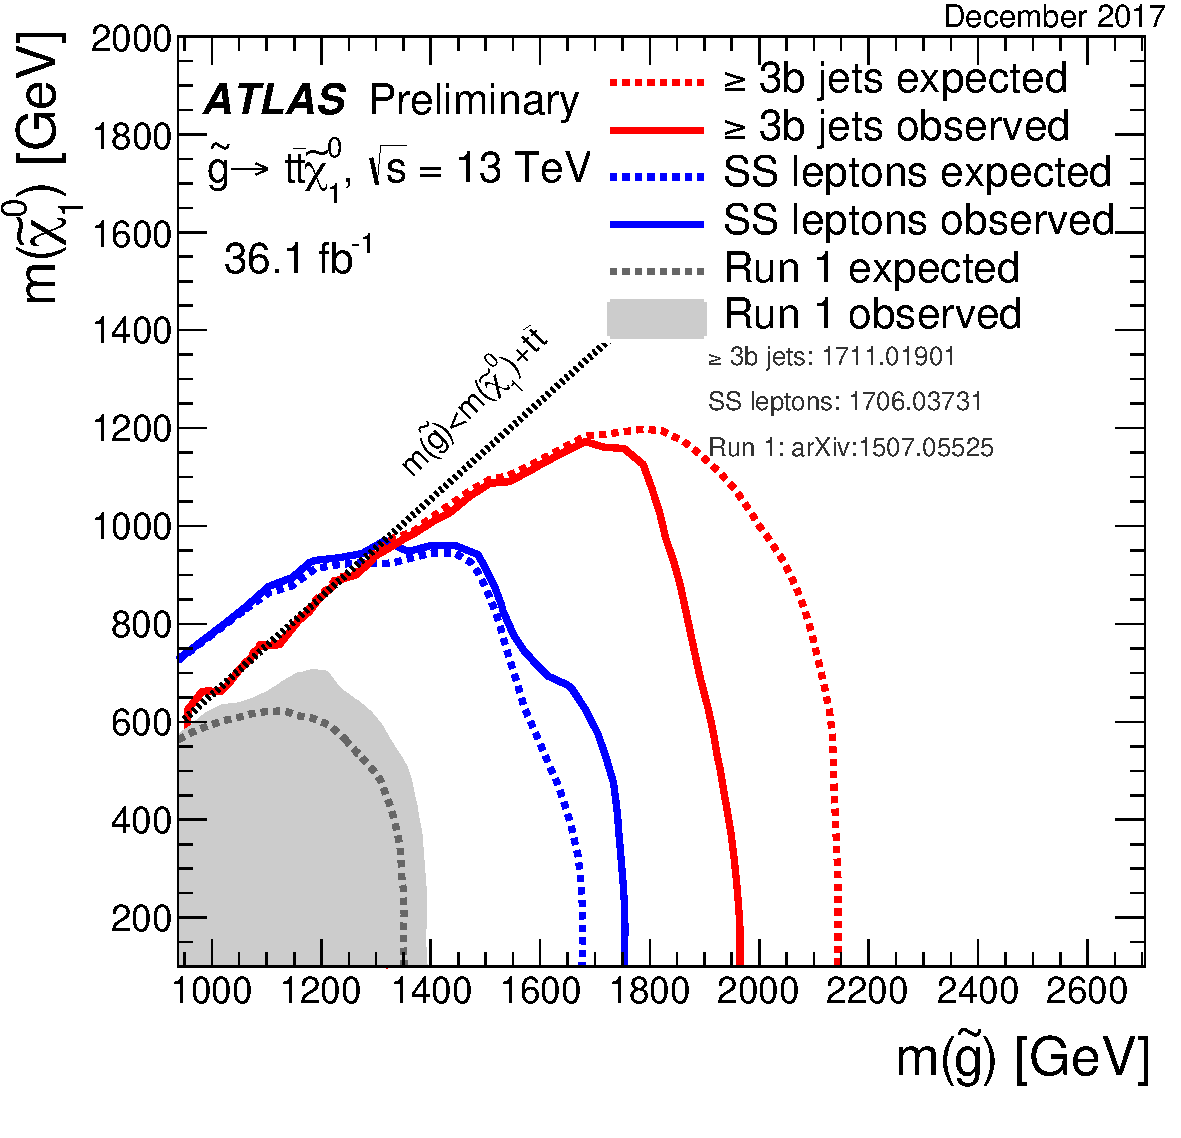
\includegraphics[width=0.45\textwidth]{figures/summary_plots/ATLAS_SUSY_Gtt.pdf}
	\caption{Exclusion limits at 95\% CL based on 13 TeV data in the (gluino, lightest neutralino) 
	mass plane for the Gtt simplified model where a pair of gluinos decays promptly via off-shell top 
	squarks to four top quarks and two lightest neutralinos. Theoretical signal cross section uncertainties are 
	not included in the limits shown. Figure from Ref. \cite{atlasSUSYSummary}.
	} 
	\label{fig:summary_atlas_Gtt}
\end{figure}

In the case of the \gls{cms} Collaboration, several analyses provide an interpretation for both the Gtt and 
the Gbb signal models, shown respectively in Figures \ref{fig:limits_Gtt_cms} and \ref{fig:limits_Gbb_cms}.
The \htmiss analysis \cite{Sirunyan:2017cwe} provides the best sensitivity for both models in the case of massless 
neutralino; this analysis performs a four-dimensional scan of zero-lepton events with at least two jets, binning them 
based on the scalar sum of the \pt of the signal jets in the event (\Ht), the negative vector sum of the jets (\htmiss), 
the number of jets and the number of b-jets. 

In the case of the Gtt model, for high gluino mass and intermediate neutralino mass the most sensitive analysis is
the 0-lepton analysis with reconstructed hadrinically decaying top quarks \cite{Sirunyan:2017pjw}, 
that builds several \glspl{sr} based on the number of jets, the number of b-jet, the number of reconstructed top quark 
candidates, \met, \Ht and \mttwo, a transverse-mass type variable designed to reduce the \ttbar background. 
For signal models with small mass difference between the gluino and the neutralino, the most sensitive analysis 
is also for \gls{cms} the same-sign analysis \cite{Sirunyan:2017uyt}, that selects events with two leptons with 
the same charge and builds several \glspl{sr} based on number of jets, number of b-jets, \met, \Ht, and \mt. 

The \mttwo analysis \cite{Sirunyan:2017kqq}, that uses 0-lepton events with high \mttwo,
 is the one most sensitive for Gbb models with high gluino mass 
and intermediate neutralino mass. 
The Gbb signal does not produce any prompt lepton, so in this case also when the neutralino mass approaches the kinematic 
limit it is a 0-lepton analysis that provides the best sensitivity: 
in the \alphat analysis \cite{Sirunyan:2018vjp}, all the \glspl{sr} are defined in the phase-space region 
with large \alphat, defined as the ration between the energy of the sub-leading jet and the transverse mass
between the leading and subleading jet. 

\begin{figure}[htbp]
	\centering 
	\subfigure[]{\includegraphics[width=0.49\textwidth]{figures/cms/T1tttt_limits_summary_cms.pdf}\label{fig:limits_Gtt_cms}}
	\subfigure[]{\includegraphics[width=0.49\textwidth]{figures/cms/T1bbbb_limits_summary_cms.pdf}\label{fig:limits_Gbb_cms}}
	\caption{Mass limits at 95\% CL obtained for simplified models of gluino pair production 
	with gluino decays to \subref{fig:limits_Gtt_cms} pairs of top quarks and the LSP and \subref{fig:limits_Gbb_cms}
	pairs of bottom quarks and the LSP. 
	In the figures, the solid (dashed) 
	lines correspond to the observed (median expected) limits. The arXiv numbers corresponding to the different analyses are shown in the legend.
	}
	\label{fig:limits_GbbGtt_comp}
\end{figure}

\FloatBarrier

\section{RPV interpretation}

Throughout this thesis, only models with R-parity conservation have been considered. 
 

\begin{figure}[htbp]
	\centering 
	\subfigure[]{\includegraphics[width=0.32\textwidth]{figures/rpv/fig_01d.pdf}}
	\subfigure[]{\includegraphics[width=0.32\textwidth]{figures/rpv/fig_01e.pdf}}
	\subfigure[]{\includegraphics[width=0.32\textwidth]{figures/rpv/fig_01f.pdf}}
	\caption{Production and decay process for the \gls{rpv} Gtt model considered.
	 The dominant process varies with increasing $\lambda''$ coupling from left to right.}
	\label{fig:rpcrpv_diagrams}
\end{figure}

\begin{figure}[htbp]
	\centering
	\includegraphics[width=0.65\textwidth]{figures/rpv/fig_04.pdf}
	\caption{	
	Exclusion limits for the Gtt model as a function of $\lambda_{323}''$ and m($\tilde{g}$). Expected limits are shown with dashed lines, and observed as solid. The \gls{rpcsusy}-limit is shown on the leftmost part of the axes, while the region $\lambda_{323}''>$ 1.07 is forbidden by constraints from the renormalization group equations. Figure from Ref. \cite{ATLAS-CONF-2018-003}.
	} 
	\label{fig:rpv_Gtt}
\end{figure}

\FloatBarrier

\section{Higgsino pair production in GMSB models}

The exclusion contours in the plane of \mhino-\gls{br} plane are shown in Figures \ref{fig:summary_atlas_higgsino_GMSB} 
and \ref{fig:limits_higgsino_cms} for the \gls{atlas} and \gls{cms} collaborations respectively.

\begin{figure}[htbp]
	\centering
	\includegraphics[width=0.65\textwidth]{figures/summary_plots/ATLAS_SUSY_EWSummary_GGM.pdf}
	\caption{The 95\% CL exclusion limits on a general gauge mediation model from 13 TeV data. 
	The model assumes a pure Higgsino NLSP that promptly decays to either Z gravitino or Higgs gravitino. 
	The limits are displayed as a function of the mass of the nearly mass-degenerate Higgsino triplet and the branching fraction of lightest Higgsino to Higgs gravitino. 	Figure from Ref. \cite{atlasSUSYSummary}.
	} 
	\label{fig:summary_atlas_higgsino_GMSB}
\end{figure}

The \gls{cms} collaboration has a more extensive program covering this signal model for what concerns the analysis of the 
2015-2016 dataset. 
Different final states are exploited to be sensitive to the possible combinations of branching ratios, 
providing a good sensitivity throughout the full plane: 
the expected sensitivity is up to about 580 GeV in the case $B(\hino\rightarrow Z \tilde{G})=100$\% and 800 GeV for 
$B(\hino\rightarrow h \tilde{G})=100$\%.

\begin{figure}[htbp]
	\centering 
	\subfigure[]{\includegraphics[width=0.49\textwidth]{figures/cms/CMS-SUS-17-004_Figure_011.pdf}\label{fig:limits_higgsino_cms_comb}}
	\subfigure[]{\includegraphics[width=0.49\textwidth]{figures/cms/CMS-SUS-17-004_Figure_012.pdf}\label{fig:limits_higgsino_cms_individual}}
	\caption{
	Exclusion contours at the 95\% CL in the plane of m(\ninoone) and \gls{br}(\ninoone $\to$ H \gravino) for the model of \ninoone\ninoone production.
    \subref{fig:limits_higgsino_cms_comb}     
	Combined exclusion contours. The area to the left of or below the solid (dashed) black curve represents the observed (expected) exclusion region. The green and yellow bands indicate the $\pm1$ and $2\sigma$ uncertainties in the expected limit. The thin black lines show the effect of the theoretical uncertainties ($\pm1\sigma_{theory}$) on the signal cross section.
	\subref{fig:limits_higgsino_cmsindividual}
	Observed contours for each individual analysis compared with the combination. For the 4b contour, the region above is excluded, while for all others, the region to the left is excluded. The 4b search drives the exclusion at large values of \gls{br}(\ninoone $\to$ H \gravino) while the on-Z dilepton and multilepton searches are competing at lower values of \gls{br}(\ninoone $\to$ H \gravino).
		}
	\label{fig:limits_higgsino_cms}
\end{figure}

\FloatBarrier


\section{ATLAS mass reach}

\begin{figure}[htbp]
	\centering
	\includegraphics[width=1\textwidth]{figures/summary_plots/ATLAS_SUSY_Summary.pdf}
	\caption{	Mass reach of the ATLAS searches for Supersymmetry. 
	A representative selection of the available search results is shown. Results are quoted for the nominal cross section 
	in both a region of near-maximal mass reach and a demonstrative alternative scenario, in order to display the range in 
	model space of search sensitivity. Some limits depend on additional assumptions on the mass of the intermediate states, 
	as described in the references provided in the plot. Figure from Ref. \cite{atlasSUSYSummary}.
	} 
	\label{fig:summary_atlas_summary}
\end{figure}